\chapter{Dise\~{n}o del Control de Estabilizaci\'{o}n} \label{sec:ControlChapter}

\section{Introducci�n}
El objetivo principal de este trabajo es implementar un control que permita la estabilizaci\'{o}n de l\'{i}nea de vista de la c\'{a}mara montada en el eslab\'{o}n interno del del sistema gimbal. El torque de control de elevaci�n $T_{el}$  y el torque de control de la elevaci�n cruzada $T_{az}$ pueden ser generados por diferentes algoritmos, pero indiferentemente del algoritmo el principal objetivo del sistema de control es suprimir cualquier efecto provocado por el movimiento del aeronave, es decir $\omega_{B}$ o su derivada  $\dot{\omega}_B$. Esto se puede lograr mediante realimentaci\'{o}n directa (Estabilizaci\'{o}n Directa) o mediante la cancelaci\'{o}n de la perturbaci\'{o}n por medio de las mediciones inerciales en la base del gimbal (Estabilizaci\'{o}n Indirecta). Para el dise\~{n}o del control del sistema se ha optado por elegir el enfoque de estabilizaci\'{o}n directa, ya que en el an\'{a}lisis desarrollado por P. J. Kennedy en \cite{3}, se concluye que con el m\'{e}todo de estabilizaci\'{o}n directa se pueden obtener mejores resultados en la estabilizaci\'{o}n de la l\'{i}nea de vista. En la estabilizaci\'{o}n directa, se miden las velocidades angulares $\omega_{T_y}$ y $\omega_{T_z}$ y estas son usadas para generar los torques de compensaci�n $T_{T\omega}$ y $T_{P\omega}$, los cuales intentan anular las perturbaciones medidas, la figura ~\ref{fig:BloquesCont} muestra la configuraci\'{o}n para el lazo de control de estabilizaci\'{o}n directa.

\begin{figure}[H]
\centering
      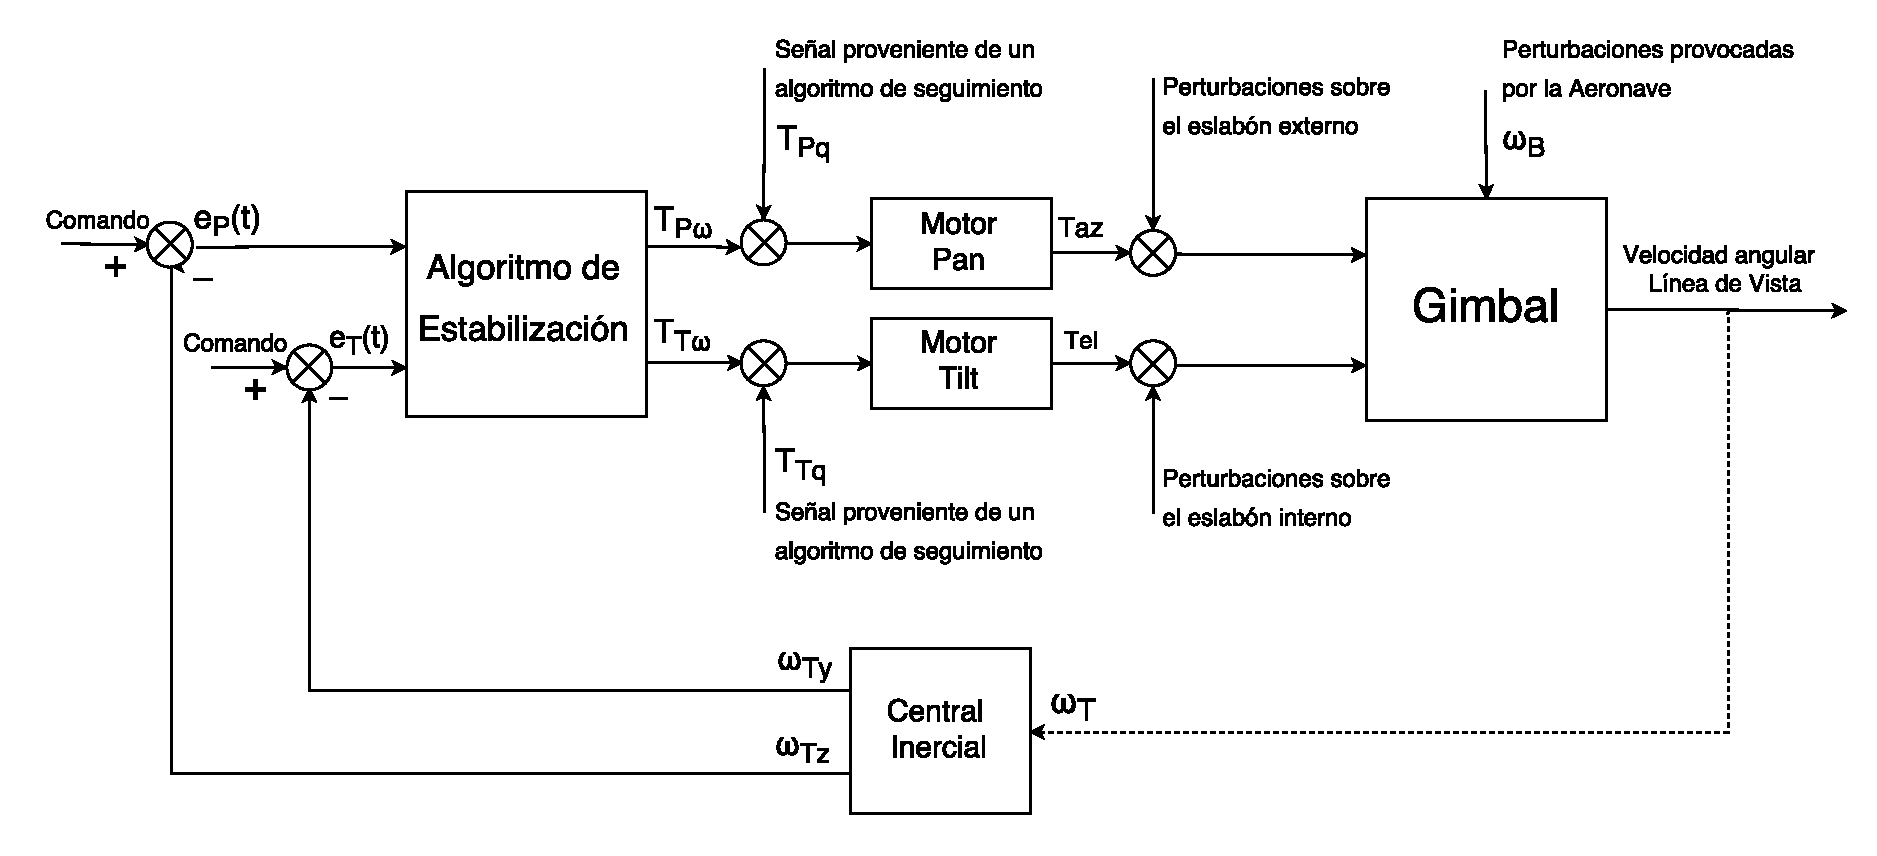
\includegraphics[scale=0.45]{img/DiagControl.pdf}
      \caption{Configuraci\'{o}n para el lazo de control de estabilizaci\'{o}n directa}
      \label{fig:BloquesCont}
\end{figure}

En la formulaci\'{o}n de cualquier problema de control siempre habr\'{a} una discrepancia entre la din\'{a}mica real del sistema y el modelo din\'{a}mico usado para dise\~{n}ar el controlador. Estas discrepancias surgen de perturbaciones externas desconocidas, par\'{a}metros de la planta, y din\'{a}micas no modeladas y parasitarias. Debido a esto se han desarrollado de m\'{e}todos de control robusto como un m\'{e}todo para compensar la inexactitud del modelado \cite{21}. Un enfoque simple del control robusto es la llamada metodolog\'{i}a de control de modos deslizantes. Intuitivamente, se basa en la observaci\'{o}n de que es mucho m\'{a}s f\'{a}cil controlar sistemas de primer orden, es decir sistemas descritos por ecuaciones diferenciales de primer orden ya sean no lineales o con incertidumbres en sus par\'{a}metros que controlar sistemas de orden \textit{n}, para lograr esto, se introduce una simplificaci\'{o}n notacional que permite reemplazar los sistemas de orden \textit{n} por problemas equivalentes de primer orden. Para los sistemas modificados, es posible probarse al menos en principio que se puede alcanzar un desempe\~{n}o \textit{"perfecto"}, en la presencia inexactitudes arbitrarias en los par\'{a}metros. Sin embargo, tal desempe\~{n} es obtenido con la consecuencia de una actividad extremadamente alta en la se\~{n}al de control (Chattering), este fen\'{o}meno es un efecto no deseado que puede generar inestabilidad en la din\'{a}mica del sistema al excitar din\'{a}micas internas no consideradas. 

En este cap\'{i}tulo se presenta el dise\~{n}o de un algoritmo de control por la metodolog\'{i}a de modos deslizantes y posteriormente se compara con un compensador PI frecuentemente usado para el control de este tipo de sistemas, con el fin de tener una referencia para medir el desempe\~{n}o del algoritmo dise\~{n}ado. Se realizan varias simulaciones elaborando un modelo en Simulink del modelo din\'{a}mico obtenido en las ecuaciones ~\ref{eq:Elev} y ~\ref{CrossEl} as\'{i} como de las leyes de control obtenidas.

 
\section{Control Sliding Mode} \label{sec:ControlSM}

El objetivo es controlar la velocidad angular sobre los ejes de elevaci\'{o}n y elevaci\'{o}n cruzada. Por consiguiente, las velocidades angulares $\omega _{T_y}$ y $\omega _{T_z}$ son las variables a controlar por el sistema de lazo cerrado. El prop\'{o}sito es mantener $\omega _{T_y}=\omega _{T_z}=0$ a pesar de las perturbaciones, y mantener sin rotaci\'{o}n el sensor con respecto al marco inercial. 

Las ecuaciones que describen el sistema gimbal bajo consideraci\'{o}n son altamente no lineales e incluyen t\'{e}rminos que no son conocidos con precisi\'{o}n o que no pueden ser medidos con precisi\'{o}n durante el vuelo. Se ha demostrado que el uso de control de estructura variable o control por modos deslizantes pueden proveer un desempe\~{n}o de seguimiento robusto en presencia de no linealidades e incertidumbres \cite{13}.


\subsection{Control de Elevaci\'{o}n}

En la secci\'{o}n ~\ref{sec:DinDes} se desarroll\'{o} la din\'{a}mica deseada para el canal de elevaci\'{o}n del sistema gimbal, la cual esta dada por la ecuaci\'{o}n ~\ref{eq:ElDinDes}. Esta ecuaci\'{o}n fue obtenida al considerar ciertas condiciones de simetr\'{i}a, bajo estas condiciones las perturbaciones inerciales desaparecen dejando \'{u}nicamente el par producido por el motor. 

Ahora para dise�ar el control podemos considerar las perturbaciones tales como la fricci\'{o}n, los pares debidos a masas no balanceadas, gradiente gravitacional, etc. como una sola perturbaci\'{o}n acotada, con lo anterior podemos reescribir la din\'{a}mica de elevaci\'{o}n como

\begin{equation}
I_{T_y}\dot{\omega}_{T_z} = T_{el} + f(x_{1_T},x_{2_T},t)
\label{eq:ContElevDina}
\end{equation}

Donde las variables de estado se definen de la siguiente manera

\begin{equation}
\begin{array}{c}
x_{1_T}=\int_0^t \! \omega _{T_y}(t) \,\mathrm{d}t \\ \\
\dot{x}_{1_T}=x_{2_T}=\omega _{T_y}
\end{array}
\label{eq:statevar}
\end{equation}

Y la funci\'{o}n $f(x_{1_T},x_{2_T},t)$ es el t\'{e}rmino de pertubaci\'{o}n el cual engloba todas las no linealidades de la ecuaci\'{o}n ~\ref{Elev_2} as\'{i} como cualquier otra perturbaci\'{o}n no considerada en el modelado. Se asume que esta funci\'{o}n esta acotada de tal manera que $\abs{f(x_{1_T},x_{2_T},t)} \leq L > 0$ y esta dada por

\begin{equation}
\begin{array}{cl}
f(x_{1_T},x_{2_T},t) = & -k_{Tvf} \, \omega_{T_y} + \left[ t\varepsilon \, \left(I_{T_x}-I_{T_z}\right) \right]\omega_{T_y}^2 + \\
 &\left[ \frac{1}{c \varepsilon} \left(I_{T_z}-I_{T_x}\right) \right] \left[ c \eta \omega_{B_x} \omega _{T_z} + s \eta \omega_{B_y} \omega _{T_z} \right] + k_{Tvf} \, \left[ c \eta \omega_{B_y} - s \eta \omega_{B_x} \right] \\
 & -  k_{Tcf} \, \mathrm{sign}\left( \omega_{T_y} - c \eta \omega_{B_y} + s \eta \omega_{B_x} \right) + T_{U_{Ty}}
\end{array}
\label{eq:fxT}
\end{equation}

Ahora usando las definiciones de las variables de estado dadas en ~\ref{eq:statevar}, podemos transformar la ecuaci\'{o}n ~\ref{eq:ContElevDina} en su representaci\'{o}n en variables de estado

\begin{equation}
\dot{x}_{2_T}=\frac{1}{I_{T_y}}T_{el} + f(x_{1_T},x_{2_T},t)
\end{equation}

Si elegimos $T_{el}=I_{T_y}u_T$ donde $u_T$ es una entrada de control equivalente, la din\'{a}mica resultante es

\begin{equation}
\overset{.}{x}_{2_T}= u_T + f(x_{1_T},x_{2_T},t)
\end{equation}

Ahora definimos la superficie de deslizamiento, como

\begin{equation}
\sigma_{T}=c_{T}x_{1_T} + x_{2_T}, \, c>0
\end{equation}

A fin de lograr la convergencia asint\'{o}tica de las variables de estado $x_{1_T}$, $x_{2_T}$ en la presencia de la perturbaci\'{o}n acotada $f(x_{1_T},x_{2_T},t)$, aplicaremos Lyapunov a la din\'{a}mica de $\sigma_{T}$, derivando obtenemos

\begin{equation}
\dot{\sigma}_{T}=c_{T}x_{2_T}+ f(x_{1_T},x_{2_T},t)+u_T,\, \sigma_{T}(0)=0
\label{eq:sigma_dot}
\end{equation}


La siguiente funci\'{o}n candidata de Lyapunov se elije para probar la estabilizaci\'{o}n de la din\'{a}mica de $\sigma$

\begin{equation}
\mathrm{V}=\frac{1}{2}\sigma_{T}^2
\end{equation}

A fin de proporcionar estabilidad asint\'{o}tica de ~\ref{eq:sigma_dot} alrededor del punto de equilibrio $\sigma_{T}=0$, las siguientes condiciones deben satisfacerse 

\begin{enumerate}[a)]
 \item{$\dot{\mathrm{V}}<0$ para $\sigma_{T} \neq 0$}
 \item{$\lim_{\abs{\sigma_{T}} \to \infty }\mathrm{V}= \infty$}
\end{enumerate}


La condici\'{o}n (b) obviamente, se satisface con $\mathrm{V}$. A fin de lograr la convergencia en tiempo finito, la condici\'{o}n (a) puede ser modificada para ser 

\begin{equation}
\dot{\mathrm{V}} \leq - \alpha \mathrm{V}^{1/2}, \, \alpha < 0
\end{equation}


Calculando la derivada de $\mathrm{V}$, obtenemos

\begin{equation}
\overset{.}{\mathrm{V}}=\overset{.}{\sigma_{T}}\sigma_{T} = \sigma_{T} \left( c_{T}x_{2_T} + f(x_{1_T},x_{2_T},t) + u_T \right)
\end{equation}


Asumiendo que $u_T=-c_{T}x_{2_T}+v$ y sustituyendo en la expresi\'{o}n anterior, obtenemos

\begin{equation}
\begin{array}{cl}
\dot{\mathrm{V}}= & \sigma_{T} \left( f(x_{1_T},x_{2_T},t)+ v \right) \\
                  & \sigma_{T} f(x_{1_T},x_{2_T},t) + \sigma_{T} v \leq \abs{\sigma_{T}} L + \sigma_{T} v
\end{array}
\label{eq:V_dot}
\end{equation}

Eligiendo $v=-\rho_{T} \, \mathrm{sign} \left( \sigma_{T} \right)$, donde

\begin{equation}
\mathrm{sign}(x) = \begin{cases} 1 &\mbox{if } x > 0 \\
 0 &\mbox{if } x = 0 \\
-1 & \mbox{if } x < 0. \end{cases}
\end{equation}

Con $\rho_{T} > 0$ y substituyendo en ~\ref{eq:V_dot}, obtenemos

\begin{equation}
\dot{\mathrm{V}} \leq \abs{\sigma_{T}}L - \rho_{T} \abs{\sigma_{T}} = -\abs{\sigma_{T}} \left( \rho_{T} -L \right)
\label{eq:V_dot_2}
\end{equation}

Podemos ver de ~\ref{eq:V_dot_2} que mientras $\rho_{T} > L$ la estabilidad esta garantizada. Por lo tanto, finalmente la ley de control para el canal de elevaci\'{o}n es

\begin{equation}
T_{el}=I_{T_y} \left( -c_{T}\omega_{T_y} - \rho_{T} \, \mathrm{sign} \left( \sigma_{T} \right) \right)
\label{eq:ElevControlSM}
\end{equation}


\subsection{Control de Elevaci\'{o}n Cruzada}

Al igual que con la din\'{a}mica de elevaci\'{o}n, consideraremos a las perturbaciones inerciales, el par causado por la fricci\'{o}n, y las din\'{a}micas no modeladas, como una sola perturbaci\'{o}n acotada $f(x_{1_P},x_{2_P},t)$, reescribiendo la ecuaci\'{o}n ~\ref{CrossEl}, tenemos

\begin{equation}
Js\dot{\omega}_{T_z} = c\varepsilon T_{az} + f(x_{1_P},x_{2_P},t)
\end{equation}

donde

\begin{equation}
\begin{array}{c}
x_{1_P}=\int_0^t \! \omega _{T_z}(t) \,\mathrm{d}t \\ \\
\dot{x}_{1_P}=x_{2_P}=\omega _{T_z}
\end{array}
\label{eq:statevarAz}
\end{equation}

Son las variables de estado y la funci\'{o}n $f(x_{1_P},x_{2_P},t)$ es el t\'{e}rmino de pertubaci\'{o}n el cual engloba todas las no linealidades de la ecuaci\'{o}n ~\ref{CrossEl} as\'{i} como cualquier otra perturbaci\'{o}n no considerada en el modelado. Se asume que esta funci\'{o}n esta acotada de tal manera que $\abs{f(x_{1_P},x_{2_P},t)} \leq L_P > 0$.

Siguiendo el mismo proceso que para el dise\~{n}o del control de elevaci\'{o}n, obtenemos la ley de control para el canal de acimut o elevaci\'{o}n cruzada, dado por

\begin{equation}
T_{az}=\frac{Js}{c\varepsilon} \left( -c_{P}\omega_{T_z} - \rho_{P} \, \mathrm{sign} \left( \sigma_{P} \right) \right)
\end{equation}


\subsection{Reducci\'{o}n del Efecto "Chattering"} \label{sec:ChatRed}

En los sistemas de control de motores CD, es importante evitar el effecto de casta\~{n}eo o \textit{"chattering"} al proveer se�ales de control continuas y suaves. Una soluci\'{o}n para lograr esto, es aproximar la funci\'{o}n discontinua $\mathrm{sign}(x)$ a alguna alternativa continua. Por ejemplo, puede ser reemplazada por una funci\'{o}n sigmoide\cite{21}, dada por

\begin{equation}
\mathrm{sign}(x) \approx \frac{x}{\abs{x}+\epsilon}
\label{eq:sigmoide}
\end{equation}

Donde $\epsilon$ es un escalar peque\~{n}o y positivo, tal que

\begin{equation}
\lim_{\epsilon \to 0}\frac{x}{\abs{x}+\epsilon}=\mathrm{sign}(x); \, x \neq 0
\end{equation}


\section{Compensador Proporcional-Integral}

Tal como se menciona en \cite{6}, el controlador PID convencional y sus constructores (P, PI y PD) son los algoritmos m\'{a}s utilizados debido a su estructura simple, bajo costo, dise�o simple y alto desempe\~{n}o, siendo el compensador proporcional-integral (PI) un algoritmo frecuentemente utilizado para el control de sistemas de estabilizaci\'{o}n inercial \cite{3}. Es por este motivo que este m\'{e}todo de control se utilizar\'{a} como un punto de referencia para medir el desempe\~{n}o del algoritmo de control robusto dise\~{n}ado en la secci\'{o}n anterior ~\ref{sec:ControlSM}. Las ecuaciones del compensador proporcional-integral para el canal de elevaci\'{o}n y elevaci\'{o}n cruzada se muestran en ~\ref{eq:ContPIElev} y ~\ref{eq:ContPICross} respectivamente.

\begin{equation}
T_{el}=-\left(K_{P_{el}}\omega_{T_y}+ K_{I_{el}} \int_{0}^{t} \! \omega _{T_y}(\tau) \,\mathrm{d}\tau  \right)
\label{eq:ContPIElev}
\end{equation}

\begin{equation}
T_{az}=-\left(K_{P_{az}}\omega_{T_z}+ K_{I_{az}} \int_{0}^{t} \! \omega _{T_z}(\tau) \,\mathrm{d}\tau  \right)
\label{eq:ContPICross}
\end{equation}
\newpage

\section{Simulaciones}

El modelo desarrollado en la secci\'{o}n ~\ref{sec:Modelado}, definido por la ecuaciones ~\ref{Elev_2} y ~\ref{CrossEl}, se construye en el entorno de simulaci\'{o}n Simulink\textsuperscript{\textregistered} de MATLAB\textsuperscript{\textregistered}, figura~\ref{fig:GimbalSimulink}, con el prop\'{o}sito de obtener una comparaci\'{o}n cuantitativa entre el algoritmo de estabilizaci\'{o}n por modos deslizantes dise\~{n}ado en este cap\'{i}tulo y un compensador proporcional-integral com\'{u}nmente usado para estos sistemas. Para la obtenci\'{o}n de los par\'{a}metros inerciales del sistema se realiz\'{o} un modelo detallado en 3D empleando el programa SolidWorks\textsuperscript{\textregistered}, con esta herramienta fue posible obtener una aproximaci\'{o}n del valor de la matriz de inercia necesaria para la simulaci\'{o}n. Los par\'{a}metros inerciales para el eslab\'{o}n interno y externo se muestran en la tabla ~\ref{Table:IGparameters}. 

\begin{figure}[H]
      \centering
      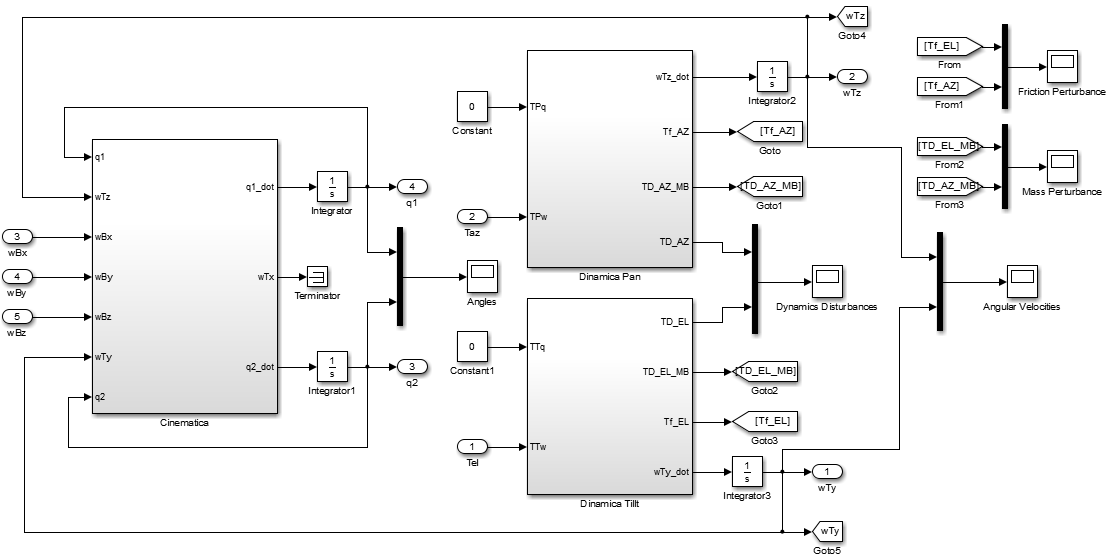
\includegraphics[scale=0.5]{Img/GimbalSimulink.png}
      \caption{Simulation Block Diagram}
      \label{fig:GimbalSimulink}
\end{figure}

\begin{table}[H]
\caption{Par\'{a}metros Inerciales del Eslab\'{o}n Interno}
\label{Table:IGparameters}
\begin{center}
\begin{tabular}{ |c|c| }
\hline
\multicolumn{2}{ |c| }{\textbf{Par\'{a}metros Inerciales Eslab\'{o}n Interno}} \\
\hline
\textit{Variable} & \textit{Valor} \\
\hline
$I_{T_x}$ & $1.68\e{-4} \left(kg \cdot m^2\right)$  \\
$I_{T_y}$ & $1.78\e{-4} \left(kg \cdot m^2\right)$  \\
$I_{T_z}$ & $1.16\e{-4} \left(kg \cdot m^2\right)$  \\
 \hline
 \multicolumn{2}{ |c| }{\textbf{Par\'{a}metros Inerciales Eslab\'{o}n Externo}} \\
\hline
\textit{Variable} & \textit{Valor} \\
\hline
$I_{P_x}$ & $2.62\e{-3} \left(kg \cdot m^2\right)$  \\
$I_{P_y}$ & $2.47\e{-3} \left(kg \cdot m^2\right)$  \\
$I_{P_z}$ & $4.66\e{-4} \left(kg \cdot m^2\right)$  \\
\hline
\end{tabular}
\end{center}
\end{table}

Como se detalla en la secci\'{o}n ~\ref{sec:Implementacion} en el prototipo se utilizan baleros tipo bola de alta precision para la construcci\'{o}n del gimbal, lo cual permite reducir el efecto de la fricci\'{o}n al m\'{i}nimo,  Los par\'{a}metros de los coeficientes de fricci\'{o}n para la simulaci\'{o}n se obtienen de la literatura \cite{3}, \cite{24} y se muestran en la tabla ~\ref{Table:FrictionParameters} 

\begin{table}[H]
\caption{Coeficientes de Fricci\'{o}n}
\label{Table:FrictionParameters}
\begin{center}
\begin{tabular}{ |c|c| }
\hline
 \multicolumn{2}{ |c| }{\textbf{Coeficientes de Fricci\'{o}n para el Eslab\'{o}n Interno y Externo}} \\
\hline
\textit{Variable} & \textit{Valor} \\
\hline
$k_{Tvf}$, $k_{Pvf}$ & $5.2\e{-3} \left(N \cdot m/rad/s\right)$  \\
$k_{Tcf}$, $k_{Pcf}$ & $3.6\e{-3} \left(unit-less\right)$  \\
\hline
\end{tabular}
\end{center}
\end{table}

En la tabla~\ref{table:Bparameters} se muestran las se�ales de perturbaci\'{o}n empleadas para la simulaci\'{o}n del sistema de control, estas se\~{n}ales sinusoidales se emplean en todas las simulaciones para tener uniformidad al probar los algoritmos de control propuestos. Estas se�ales simulan las posibles velocidades angulares que el aeronave experimentar\'{i}a en roll pitch y yaw durante el vuelo. En la figura ~\ref{fig:PerturbacionesBase} se muestran las gr\'{a}ficas correspondientes a estas se\~{n}ales. 


\begin{table}[H]
\caption{Se�ales de Perturbaci\'{o}n al Sistema}
\label{table:Bparameters}
\begin{center}
\begin{tabular}{ |c|c|c| }
\hline
\multicolumn{3}{ |c| }{\textbf{Se\~{n}ales de Perturbaci\'{o}n}} \\
\hline
\textit{Variable} & \textit{Amplitud} & \textit{Frecuencia} \\
\hline
$\omega _{Bx}$ & $1.5 \left(rad/seg\right)$ & $0.1 \left(Hz\right)$ \\
$\omega _{By}$ & $0.2 \left(rad/seg\right)$ & $0.3 \left(Hz\right)$  \\
$\omega _{Bz}$ & $0.8 \left(rad/seg\right)$ & $1 \left(Hz\right)$  \\
 \hline
\end{tabular}
\end{center}
\end{table}

\begin{figure}[H]
      \centering
      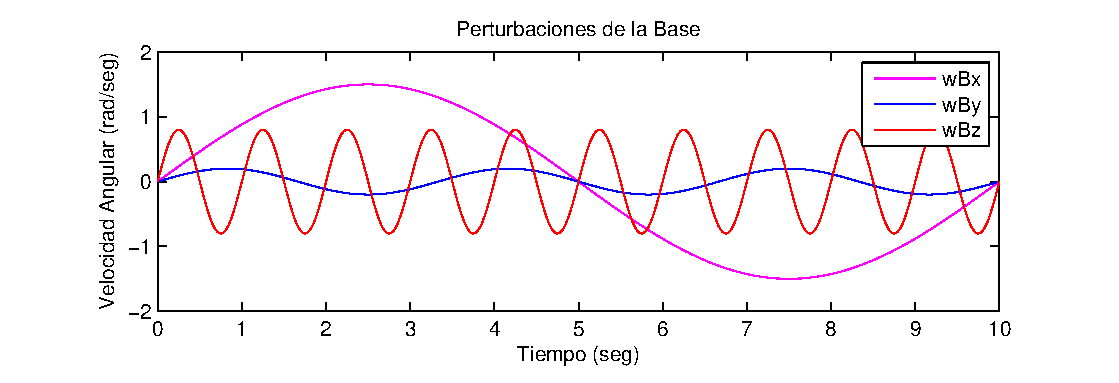
\includegraphics[scale=0.9]{Img/BasePerturbance.eps}
      \caption{Perturbaciones de la Base}
      \label{fig:PerturbacionesBase}
\end{figure} 

En la figura ~\ref{fig:ChatRed}-a podemos observar los cambios de alta frecuencia y amplitud finita propios del control por modos deslizantes, estos cambios se presentan cuando el sistema alcanza la superficie de deslizamiento y es un efecto no deseado en el control de motores DC, adem\'{a}s de que el ata actividad del control puede excitar din\'{a}micas parasitarias en el sistema. Para evitar este efecto, se emplea una funci\'{o}n sigmoide tal como se detalla en la secci\'{o}n ~\ref{sec:ChatRed}. En la figura ~\ref{fig:ChatRed}-b podemos observar la reducci\'{o}n del efecto chattering gracias al uso de la funci\'{o}n sigmoide ~\ref{eq:sigmoide} con un valor de $\epsilon=0.001$.

\begin{figure}[H]
      \centering
      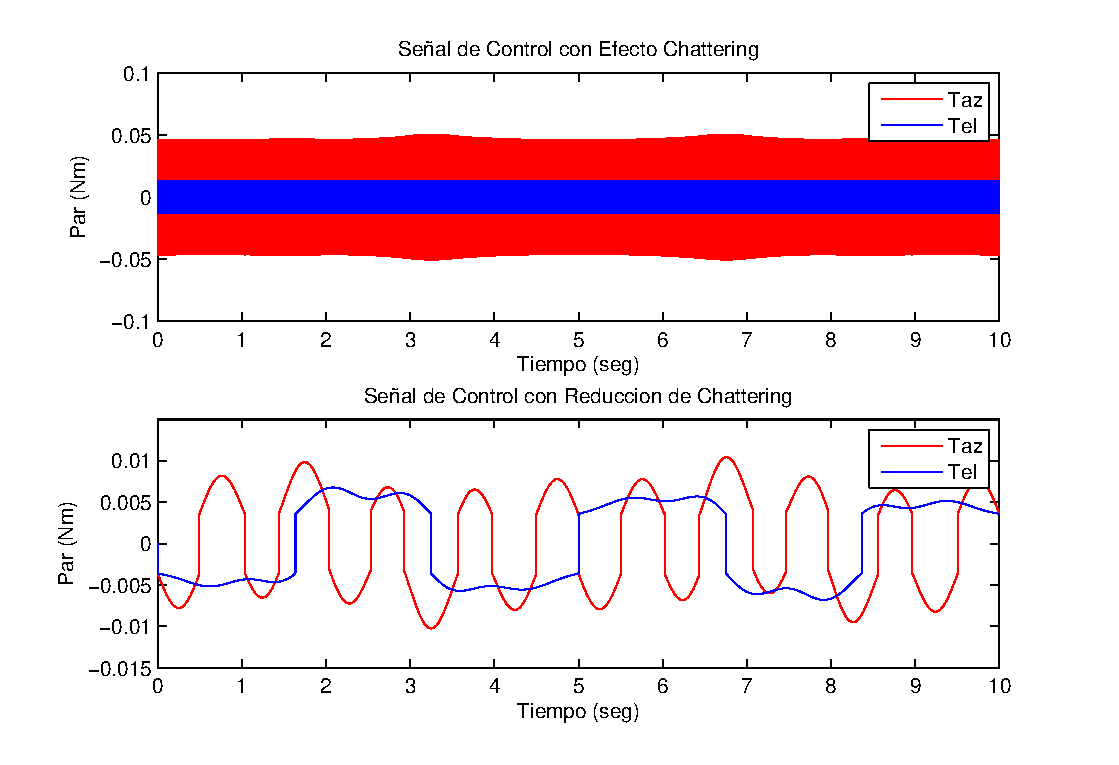
\includegraphics[scale=0.9]{img/ChatteringRed.eps}
      \caption{Reducci\'{o}n del Efecto Chattering}
      \label{fig:ChatRed}
\end{figure} 

En la figura ~\ref{fig:ContrAcc} podemos apreciar una comparaci\'{o}n entre la ley de control por modos deslizantes con dise\~{n}ada y el compensador proporcional-integral, esta comparaci\'{o}n se realiza debido a que como se ha mencionado anteriormente, los controladores PID y sus constructores siguen siendo muy utilizados debido a su simple dise\~{n}o , alto desempe\~{n}o y bajo costo, siendo el compensador PI frecuentemente utilizado para el control de este tipo de sistemas \cite{3}. La figura ~\ref{fig:ContrAcc}-a muestra la respuesta del sistema al control por modos deslizantes dise\~{n}ado, mientras que en en la figura ~\ref{fig:ContrAcc}-b se muestra la respuesta al compensador PI, podemos observar que ambos controles tienen un buen desempe\~{n}o ya que ambos son capaces de cancelar las perturbaciones del movimiento de la base, sin embargo podemos observar que el algoritmo dise\~{n}ado tiene un mejor desempe\'{n}o en la convergencia de las variables controladas $\omega _{T_y}$ y $\omega _{T_z}$.

\begin{figure}[H]
      \centering
      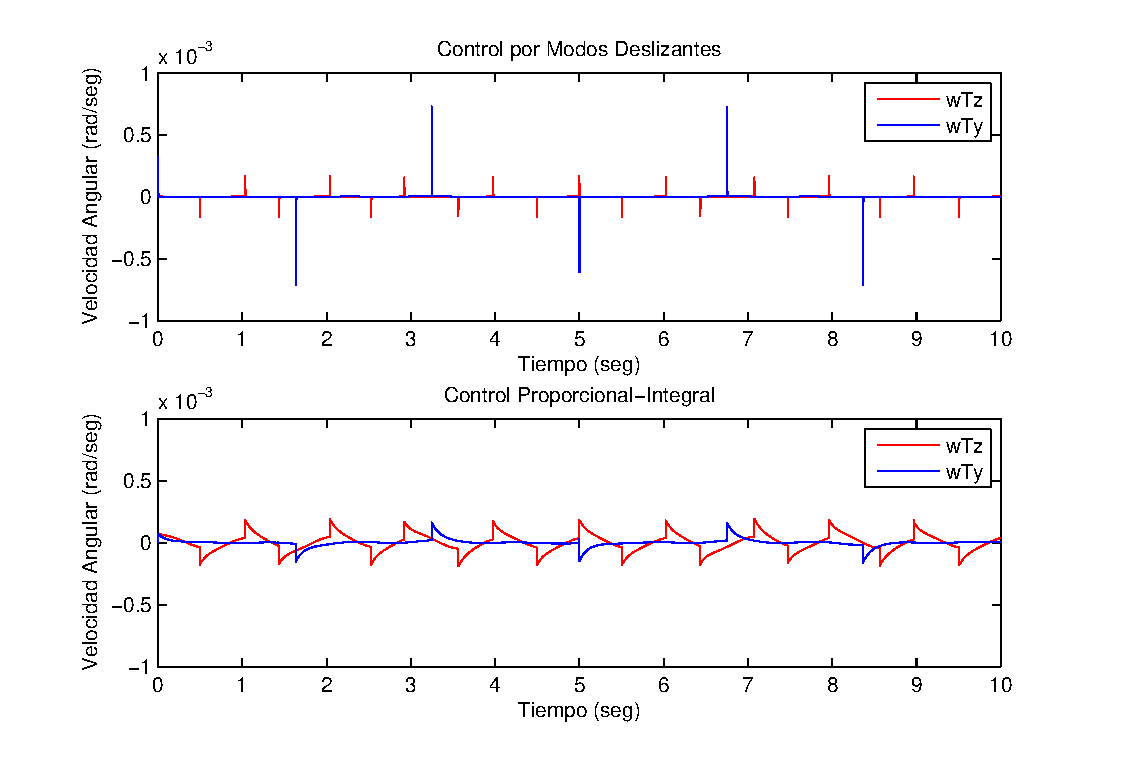
\includegraphics[scale=0.9]{img/VelAngular.eps}
      \caption{Acci\'{o}n de Control del Algoritmo de Modos Deslizantes vs Compensador PI}
      \label{fig:ContrAcc}
\end{figure}

La figura ~\ref{fig:SenalCont} muestra las se\~{n}ales de control del algoritmo por modos deslizantes y el compensador PI. Las se\~{n}ales de control del control por modos deslizantes de muestra en la figura ~\ref{fig:SenalCont}-a, mientras que la se\~{n}al de control del compensador PI se muestra en la figura ~\ref{fig:SenalCont}-b, Ambas se\~{n}ales son muy similares, pero las peque\~{n}as diferencias afectan la respuesta del sistema como muestra la figura ~\ref{fig:ContrAcc}. La se\~{n}al de control intenta cancelar las perturbaciones de la base del sistema, con el fin de mantener las variables controladas $\omega _{T_y}$ y $\omega _{T_z}$ iguales a cero, una de las perturbaciones que m\'{a}s afectan el desempe\~{n}o del sistema es el par provocado por la fricci\'{o}n tal como se menciona en \cite{10} especialmente durante los cambios de direcci\'{o}n del eslab\'{o}n interno y externo, siendo una de las influencias clave en la forma de onda de la se\~{n}al de control.  

\begin{figure}[H]
      \centering
      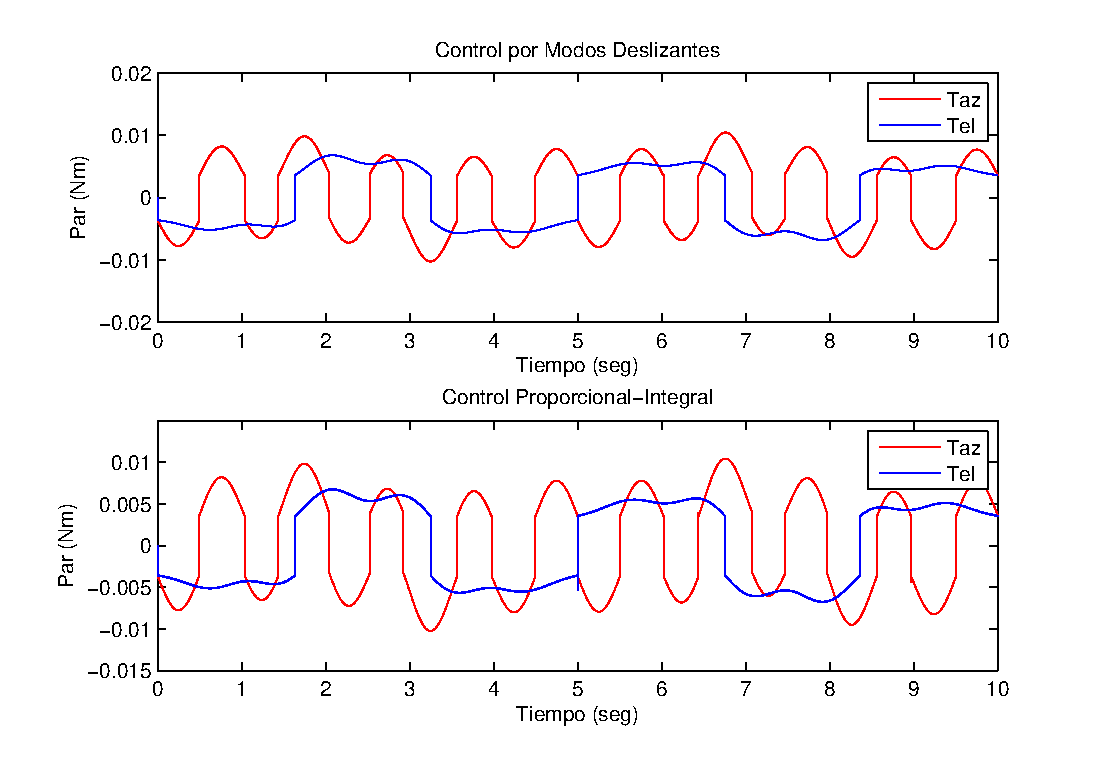
\includegraphics[scale=0.9]{img/SenalCont.eps}
      \caption{Se\~{a}l de Control del Algoritmo de Modos Deslizantes vs Compensador PI}
      \label{fig:SenalCont}
\end{figure}

Para una mejor idea de la efectividad del control dise\~{n}ado en la cancelaci\'{o}n de las perturbaciones provocadas por el movimiento del aeronave se realiza una simulaci\'{o}n en la que los primeros segundos no se aplica alg\'{u}n control y posteriormente, exactamente a los tres segundos se activa el control. En la figura ~\ref{fig:ControlEffect}-a se muestran las perturbaciones a las que esta expuesto el sistema. En la figura ~\ref{fig:ControlEffect}-b muestra las variables controladas $\omega _{T_y}$ y $\omega _{T_z}$. Podemos observar que cuando el control es activado estas r\'{a}pidamente convergen a cero y se logra la cancelaci\'{o}n de las perturbaciones de la base. Finalmente en la figura ~\ref{fig:ControlEffect}-c se muestra la variaci\'{o}n en los \'{a}ngulos del eslab\'{o}n interno y el externo para compensar el movimiento de la base.      


\begin{figure}[H]
      \centering
      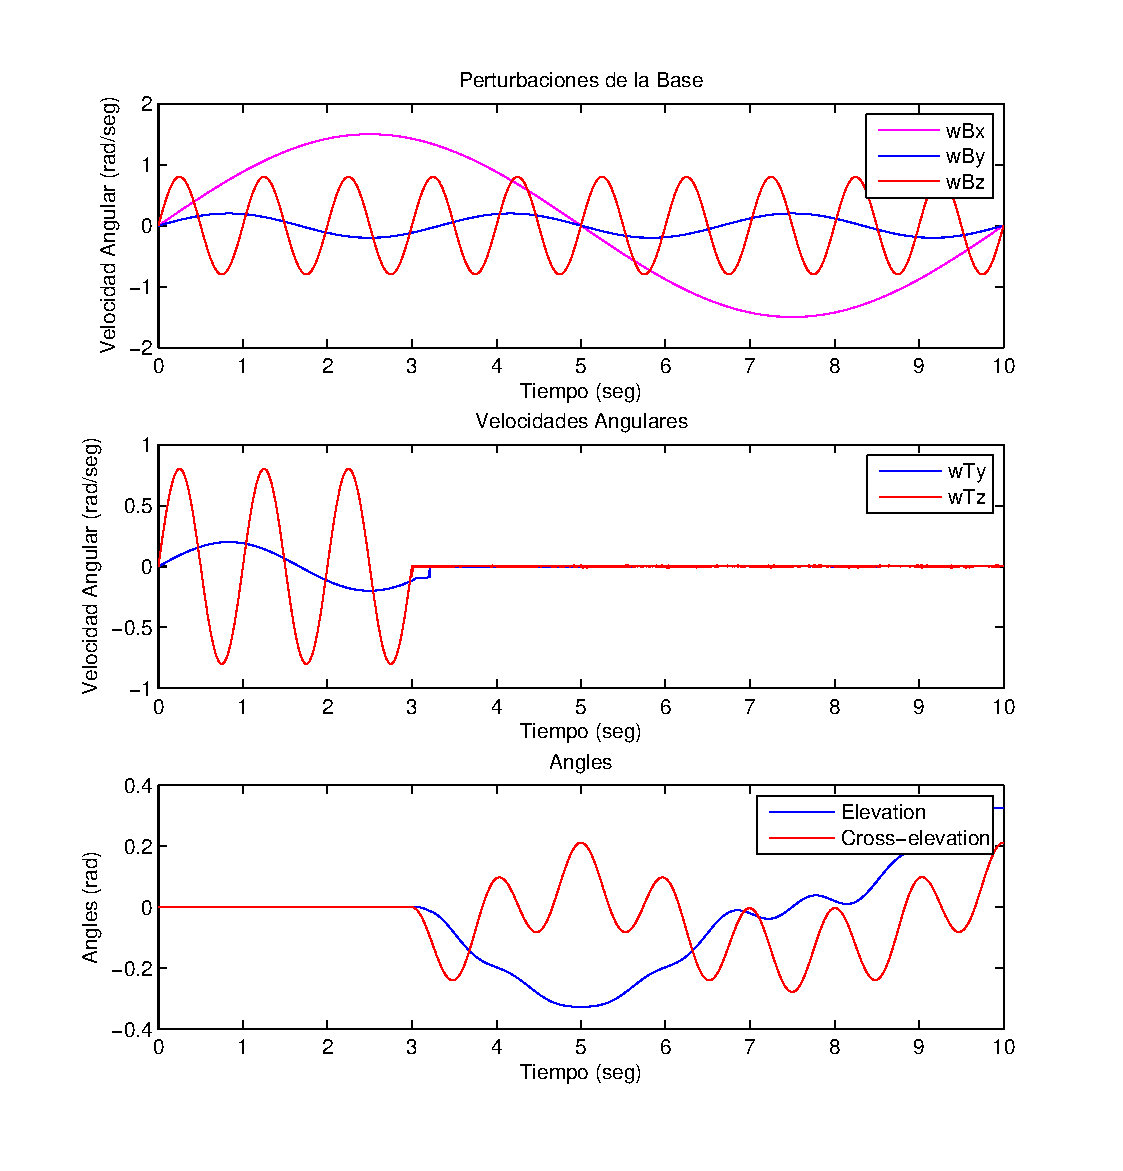
\includegraphics[scale=0.9]{img/ControlEffect.eps}
      \caption{Respuesta del Sistema al Aplicarse el Algoritmo de Estabilizaci\'{o}n}
      \label{fig:ControlEffect}
\end{figure}